\documentclass{exam-zh}
\examsetup{
  page/size=a4paper,
  page/show-head=false,
  page/show-foot=true,
  sealline/show=false,
  font=times,
  math-font=xits,
}
\usepackage{graphicx}
\usepackage{tabularx}
\usepackage{array}
\usepackage{enumitem}
\usepackage{needspace}
\usepackage[most]{tcolorbox}
\usepackage{amsmath}
\setlength{\parindent}{2em}
\setlength{\parskip}{0.2em}
\setlist[enumerate]{leftmargin=2.4em,itemsep=0.25em,topsep=0.25em}
\newcommand{\blank}[1][3cm]{\underline{\hspace{#1}}}
\newcommand{\answerarea}[1][30mm]{\par\vspace{#1}}
\newcommand{\fig}[2][0.34\linewidth]{%
  \begin{center}\includegraphics[width=#1]{figures/#2}\end{center}}
\newcommand{\fourchoices}[4]{%
  \par\noindent\begin{tabularx}{\linewidth}{@{}>{\raggedright\arraybackslash}X>{\raggedright\arraybackslash}X@{}}
  （A）#1 & （B）#2\\[0.35em]
  （C）#3 & （D）#4
  \end{tabularx}\par}
\newcommand{\twocolfig}[2]{%
  \begin{center}
  \begin{minipage}[t]{0.47\linewidth}\centering #1\end{minipage}\hfill
  \begin{minipage}[t]{0.47\linewidth}\centering #2\end{minipage}
  \end{center}}
\ifteacher
  \NewDocumentEnvironment{teachersolution}{+b}{%
    \begin{tcolorbox}[breakable,colback=gray!4,colframe=black!45,
      boxrule=0.45pt,arc=1mm,left=2mm,right=2mm,top=1.5mm,bottom=1.5mm,
      title={参考答案},fonttitle=\bfseries]#1\end{tcolorbox}}{}
  \newcommand{\studentanswer}[1]{}
\else
  \NewDocumentEnvironment{teachersolution}{+b}{}{}
  \newcommand{\studentanswer}[1]{#1}
\fi
\newcommand{\q}[1]{\par\needspace{3\baselineskip}\noindent\textbf{#1.}\enspace}
\newcommand{\subq}[1]{\par\noindent（#1）}

\begin{document}
\begin{center}
  {\zihao{2}\bfseries 初三数学期末练习卷\ifteacher（教师版）\else（学生版）\fi}\par
  \vspace{0.6em}
  姓名：\blank[3cm]\hfill 班级：\blank[2.5cm]\hfill 得分：\blank[2.5cm]
\end{center}
\vspace{0.4em}
\noindent\textbf{说明：}本练习卷共 25 题。除选择题、填空题外，其余各题须写出证明或计算的主要步骤。

\section*{一、选择题（共 24 分，每小题 4 分）}

\q{1}下列两个图形不一定是相似形的是
\fourchoices{两个圆}{两个等边三角形}{两个正方形}{两个菱形}
\begin{teachersolution}D。两个菱形的角不一定对应相等。\end{teachersolution}

\q{2}在 $\mathrm{Rt}\triangle ABC$ 中，$\angle C=90^\circ$，那么 $\sin A$ 等于
\fourchoices{$\dfrac{BC}{AC}$}{$\dfrac{AC}{BC}$}{$\dfrac{BC}{AB}$}{$\dfrac{AC}{AB}$}
\begin{teachersolution}C。$\sin A=\dfrac{\text{对边}}{\text{斜边}}=\dfrac{BC}{AB}$。\end{teachersolution}

\q{3}下列函数中，一定是二次函数的是
\fourchoices{$y=ax+1$}{$y=ax^2+1$}{$y=(a^2+1)x^2$}{$y=(ax+1)^2$}
\begin{teachersolution}C。$a^2+1>0$，二次项系数恒不为零。\end{teachersolution}

\q{4}如图 1，点 $D,E$ 分别在 $\triangle ABC$ 的边 $AB,AC$ 上，下列条件中一定能判定 $DE\parallel BC$ 的是
\fourchoices{$\dfrac{AD}{AE}=\dfrac{AB}{AC}$}{$\dfrac{DE}{BC}=\dfrac{AD}{AB}$}{$\dfrac{AD}{AC}=\dfrac{AE}{AB}$}{$\dfrac{AE}{EC}=\dfrac{AB}{BD}$}
\fig[0.26\linewidth]{fig01.png}
\begin{teachersolution}A。由 $\dfrac{AD}{AE}=\dfrac{AB}{AC}$ 得 $\dfrac{AD}{AB}=\dfrac{AE}{AC}$，由基本比例定理的逆定理知 $DE\parallel BC$。\end{teachersolution}

\q{5}如图 2，传送带和地面所成斜坡 $AB$ 的坡度为 $1:2.4$，它把物体从点 $A$ 处传送到斜坡高处，物体沿斜坡 $AB$ 方向向上所经过的路程为 26 米，那么此时物体离地面的高度为
\fourchoices{5 米}{10 米}{12 米}{13 米}
\fig[0.22\linewidth]{fig02.png}
\begin{teachersolution}B。设高为 $x$，水平长度为 $2.4x$，则斜边为 $\sqrt{x^2+(2.4x)^2}=2.6x=26$，所以 $x=10$。\end{teachersolution}

\q{6}如图 3，已知抛物线 $y=ax^2+bx+c\ (a\ne0)$ 的对称轴是直线 $x=1$，且过点 $(-1,0)$，顶点在第一象限，其部分图像如图所示。给出以下结论：① $ab<0$；② $4a+2b+c>0$；③ $3a+c>0$。其中正确的选项是
\fourchoices{①②}{①③}{②③}{①②③}
\fig[0.26\linewidth]{fig03.png}
\begin{teachersolution}A。开口向下，$a<0$；对称轴 $-\dfrac b{2a}=1$，故 $b=-2a>0$，所以 $ab<0$。图中 $x=2$ 时函数值为正，故 $4a+2b+c>0$。而 $3a+c=f(-1)=0$，③错误。\end{teachersolution}

\section*{二、填空题（共 48 分，每小题 4 分）}

\q{7}已知 $\dfrac{x}{y}=\dfrac32$，则 $\dfrac{x-y}{x+y}$ 的值是\blank。
\begin{teachersolution}$\dfrac15$。令 $x=3k,y=2k$ 即得。\end{teachersolution}

\q{8}计算：$2(\vec a-\vec b)+3\vec b=$\blank。
\begin{teachersolution}$2\vec a+\vec b$。\end{teachersolution}

\q{9}抛物线 $y=-2(x+3)^2$ 的顶点坐标是\blank。
\begin{teachersolution}$(-3,0)$。\end{teachersolution}

\q{10}如图 4，已知 $AB\parallel CD\parallel EF$，它们依次交直线 $l_1,l_2$ 于点 $A,D,F$ 和点 $B,C,E$。如果 $AD:DF=3:2$，$BC=21$，那么 $CE=$\blank。
\fig[0.24\linewidth]{fig04.png}
\begin{teachersolution}$14$。平行线分线段成比例，$\dfrac{BC}{CE}=\dfrac{AD}{DF}=\dfrac32$。\end{teachersolution}

\q{11}如图 5，从甲楼的一窗口观测点 $A$ 处测得乙楼的楼顶端 $B$ 的仰角是 $37^\circ$，那么从乙楼顶端 $B$ 处看 $A$ 处的俯角是\blank$^\circ$。
\fig[0.23\linewidth]{fig05.png}
\begin{teachersolution}$37$。两楼的水平线平行，仰角与俯角是一对内错角。\end{teachersolution}

\q{12}如图 6，在梯形 $ABCD$ 中，$AD\parallel BC$，对角线 $AC,BD$ 相交于点 $O$。如果 $\triangle BCD$ 的面积是 $\triangle ABD$ 的面积的 2 倍，那么 $\triangle BOC$ 与 $\triangle BCD$ 的面积之比是\blank。
\fig[0.24\linewidth]{fig06.png}
\begin{teachersolution}$2:3$。$S_{BCD}:S_{ABD}=BC:AD=2:1$，故 $BO:OD=BC:AD=2:1$。在 $\triangle BCD$ 中，$S_{BOC}:S_{COD}=BO:OD=2:1$，所以 $S_{BOC}:S_{BCD}=2:3$。\end{teachersolution}

\q{13}如果将抛物线 $y=x^2+2x-1$ 向上平移，使它经过点 $A(0,3)$，那么所得新抛物线的表达式是\blank。
\begin{teachersolution}$y=x^2+2x+3$。原抛物线在 $x=0$ 时 $y=-1$，需向上平移 4 个单位。\end{teachersolution}

\q{14}二次函数 $y=ax^2+bx+2$ 的自变量 $x$ 和函数值 $y$ 的部分取值如下表：
\begin{center}
\begin{tabular}{c|ccccccc}
$x$ & $\cdots$ & $-1$ & $0$ & $1$ & $2$ & $3$ & $\cdots$\\\hline
$y$ & $\cdots$ & $5$ & $2$ & $n$ & $p$ & $5$ & $\cdots$
\end{tabular}
\end{center}
那么 $n$\blank[1.5cm]$p$（填“$>$”“$<$”或“$=$”）。
\begin{teachersolution}$n<p$。由 $f(-1)=f(3)=5$，对称轴为 $x=1$，故 $n=f(1)$ 是顶点处的最小值，而 $p=f(2)>n$。\end{teachersolution}

\q{15}如图 7，监测点 $P$ 在距离道路 $l$ 的 100 米处，道路上的货车 $A$ 在监测点 $P$ 的北偏西 $60^\circ$ 的方向，道路上的汽车 $B$ 在监测点 $P$ 的东北方向。此时货车 $A$ 和汽车 $B$ 相距\blank 米（结果保留根号）。
\fig[0.27\linewidth]{fig07.png}
\begin{teachersolution}$100(\sqrt3+1)$。设 $P$ 到道路的垂足为 $H$。由题意 $PH=100$，$AH=100\tan60^\circ=100\sqrt3$，$BH=100$，故 $AB=AH+BH=100(\sqrt3+1)$。\end{teachersolution}

\q{16}广场上音乐喷泉的喷头与地面齐平，喷出的水线呈一条抛物线，水线上水珠的高度 $y$（米）关于水珠与喷头的水平距离 $x$（米）的函数解析式是 $y=-\dfrac12x^2+3x$。那么水珠从喷出到落地时的水平距离为\blank 米。
\begin{teachersolution}$6$。令 $y=0$，得 $x(-\dfrac12x+3)=0$，除去喷出点 $x=0$，落地点为 $x=6$。\end{teachersolution}

\q{17}如图 8，在 $\mathrm{Rt}\triangle ABC$ 中，$\angle ACB=90^\circ$，$\tan\angle CAB=\dfrac12$。$CD$ 平分 $\angle ACB$，$E$ 为 $DC$ 延长线上一点，且 $\angle CEA=\angle CBE$，那么 $\dfrac{CD}{CE}$ 的值为\blank。
\fig[0.26\linewidth]{fig08.png}
\begin{teachersolution}$\dfrac23$。取 $C(0,0),A(0,2),B(1,0)$，则 $\tan\angle CAB=\dfrac12$。角平分线 $CD$ 为 $y=x$，边 $AB$ 为 $y=2-2x$，故 $D(\dfrac23,\dfrac23)$。设 $E(-t,-t)\ (t>0)$，则
\[
\tan\angle CEA=\frac1{t+1},\qquad
\tan\angle CBE=\frac{t}{t+1}.
\]
由两角相等得 $t=1$。因此 $CE=\sqrt2$，$CD=\dfrac{2\sqrt2}{3}$，所以 $\dfrac{CD}{CE}=\dfrac23$。\end{teachersolution}

\q{18}如图 9，在平行四边形 $ABCD$ 中，$AB=6$，$BC=8$，$\angle B=60^\circ$，将平行四边形 $ABCD$ 绕着 $BC$ 的中点 $O$ 旋转到 $A'B'C'D'$ 的位置，当点 $B'$ 落在边 $AB$ 上时，边 $A'D'$ 与边 $CD$ 相交于点 $G$，则 $\cot\angle CGB'=$\blank。
\fig[0.27\linewidth]{fig09.png}
\begin{teachersolution}$\dfrac{\sqrt3}{6}$。按旋转后的对应边关系与平行四边形的平行关系求得 $\tan\angle CGB'=2\sqrt3$，故 $\cot\angle CGB'=\dfrac1{2\sqrt3}=\dfrac{\sqrt3}{6}$。\end{teachersolution}

\section*{三、解答题（共 78 分）}

\q{19}\textbf{（本题 10 分）}计算：$\sqrt6\cot60^\circ-|2\cos45^\circ-1|+4\sin^230^\circ$。
\studentanswer{\answerarea[45mm]}
\begin{teachersolution}
\[
\sqrt6\cdot\frac{\sqrt3}{3}-\left|2\cdot\frac{\sqrt2}{2}-1\right|+4\left(\frac12\right)^2
=\sqrt2-(\sqrt2-1)+1=2.
\]
\end{teachersolution}

\q{20}\textbf{（本题 10 分，第（1）小题 6 分，第（2）小题 4 分）}
如图 10，在 $\triangle ABC$ 中，点 $D$ 在边 $AC$ 上，且 $AD=2DC$，点 $E$ 在 $BD$ 的延长线上，$CE\parallel AB$。已知 $\overrightarrow{BA}=\vec a$，$\overrightarrow{BC}=\vec b$。
\subq{1}用向量 $\vec a,\vec b$ 分别表示向量 $\overrightarrow{AC}=$\blank，$\overrightarrow{AE}=$\blank；
\subq{2}作出向量 $\overrightarrow{AD}$ 分别在 $\vec a,\vec b$ 方向上的分向量（写出结论，不要求写作法）。
\fig[0.29\linewidth]{fig10.png}
\studentanswer{\answerarea[55mm]}
\begin{teachersolution}
（1）$\overrightarrow{AC}=\vec b-\vec a$，$\overrightarrow{AE}=-\dfrac12\vec a+\vec b$。

（2）如原参考答案图，$\overrightarrow{AM}$、$\overrightarrow{AN}$ 分别是 $\overrightarrow{AD}$ 在 $\vec a$、$\vec b$ 方向上的分向量。
\fig[0.31\linewidth]{sol20.png}
\end{teachersolution}

\q{21}\textbf{（本题 10 分，第（1）小题 6 分，第（2）小题 4 分）}
已知，如图 11，在 $\triangle ABC$ 中，点 $D,E$ 分别在边 $AB,AC$ 上，$AD\cdot AB=AE\cdot AC$，点 $F$ 是 $BE$ 与 $CD$ 的交点。
\subq{1}求证：$\triangle FDB\sim\triangle FEC$；
\subq{2}如果 $AB=15$，$AC=18$，$AD=6$，求 $EF:DF$。
\fig[0.28\linewidth]{fig11.png}
\studentanswer{\answerarea[75mm]}
\begin{teachersolution}
（1）由 $AD\cdot AB=AE\cdot AC$，得 $\dfrac{AD}{AE}=\dfrac{AC}{AB}$。又 $\angle DAC=\angle EAB$，所以 $\triangle DAC\sim\triangle EAB$，从而 $\angle ACD=\angle ABE$。于是 $\angle EFC=\angle DFB$，故 $\triangle FDB\sim\triangle FEC$。

（2）$6\times15=18\cdot AE$，得 $AE=5$，所以 $BD=9$，$EC=13$。由相似得 $\dfrac{EF}{DF}=\dfrac{EC}{BD}=\dfrac{13}{9}$，故 $EF:DF=13:9$。
\fig[0.25\linewidth]{sol21.png}
\end{teachersolution}

\q{22}\textbf{（本题 10 分，第（1）小题 4 分，第（2）小题 2 分，第（3）小题 4 分）}

\begin{tcolorbox}[colback=white,colframe=black!55,boxrule=0.5pt,arc=0mm]
\begin{center}\bfseries 拉伸运动的“密钥”\end{center}
拉伸运动对身体机能的调节起着关键作用。从运动生理学角度来看，科学的拉伸可以改善关节活动范围，提升身体的灵活性和协调性。

拉伸板是一种有效的拉伸工具，其侧面结构可以看作一个三角形（如图 12）。脚踏板 $AB$ 可绕底座铰链 $B$ 转动，支撑杆 $CD$ 的上端位于脚踏板的点 $D$ 处。通过移动支撑杆 $CD$ 下端点 $C$ 的位置，可以改变脚踏板的倾斜角度，从而调节拉伸强度。当人站在倾斜的脚踏板上时，身体重量会产生一个沿着踏板方向的拉伸力 $F$，这个力的大小决定了拉伸的强度。

拉伸力 $F$ 的大小可用公式 $F=mg\sin\alpha$ 表示，其中 $m$（单位：千克）为体重，$g\approx10$ 牛/千克，$\alpha$ 是脚踏板与水平地面之间的夹角。这个公式可以帮助我们科学地选择档位，避免过度拉伸或拉伸不足。
\fig[0.25\linewidth]{fig12.png}
\end{tcolorbox}

如图 13，小海有一款三档可调节拉伸板，三档的夹角 $\alpha$ 度数分别为 $20^\circ,25^\circ,30^\circ$。已知 $BD=30\text{ cm}$。
\subq{1}小海的体重是 50 千克，如果拉伸力 $F$ 在 180 牛至 220 牛可以达到锻炼的目的。结合计算说明，在这三档之中，小海选择哪个档位能达到锻炼的目的；
\subq{2}当档位夹角为 $30^\circ$ 时，支撑杆 $CD$ 恰好与底座 $BM$ 垂直。求此时支撑杆下端点 $C$ 与铰链 $B$ 点的距离（结果保留根号）；
\subq{3}当档位夹角从 $30^\circ$ 调到 $20^\circ$，即支撑杆的位置变化到 $D_1C_1$ 时，支撑杆 $CD$ 的端点 $D$ 在竖直方向下降约为多少厘米？
\fig[0.29\linewidth]{fig13.png}

\begin{center}
\begin{tabular}{c|cc}
$\alpha$ & $20^\circ$ & $25^\circ$\\\hline
$\sin\alpha$ & $0.34$ & $0.42$\\
$\cos\alpha$ & $0.94$ & $0.91$
\end{tabular}
\end{center}
\studentanswer{\answerarea[90mm]}
\begin{teachersolution}
（1）$F=mg\sin\alpha=50\times10\sin\alpha$。三档拉伸力依次约为 $170$ N、$210$ N、$250$ N。只有 $210$ N 落在 $180$ N 至 $220$ N 之间，所以选择 $25^\circ$ 档。

（2）在 $\mathrm{Rt}\triangle DBC$ 中，$BD=30$ cm，$\angle DBC=30^\circ$，故 $BC=BD\cos30^\circ=15\sqrt3$ cm。

（3）$30^\circ$ 档时，$DC=BD\sin30^\circ=15$ cm。作 $D_1H\perp BM$。$D_1B=DB=30$ cm，$\angle D_1BC_1=20^\circ$，所以 $D_1H=30\sin20^\circ\approx10.2$ cm。下降约 $15-10.2=4.8$ cm。
\fig[0.28\linewidth]{sol22.png}
\end{teachersolution}

\q{23}\textbf{（本题 12 分，第（1）小题 6 分，第（2）小题 6 分）}
如图 14，在 $\mathrm{Rt}\triangle ABC$ 中，$\angle BAC=90^\circ$，$AD\perp BC$，垂足为点 $D$，点 $E$ 是边 $AC$ 上一点，$EF\perp BC$，垂足为点 $F$，$AD,BE$ 交于点 $M$。
\subq{1}如果 $BE$ 平分 $\angle ABC$，求证：$BM\cdot CE=AM\cdot BE$；
\subq{2}如果 $BD=CF$，求证：$\dfrac{EF}{AD}=\dfrac{AB^2}{AC^2}$。
\fig[0.34\linewidth]{fig14.png}
\studentanswer{\answerarea[110mm]}
\begin{teachersolution}
（1）在 $\mathrm{Rt}\triangle ABC$ 中，$\angle ABC+\angle C=90^\circ$；在 $\mathrm{Rt}\triangle ABD$ 中，$\angle ABC+\angle BAM=90^\circ$，故 $\angle BAM=\angle C$。又 $BE$ 平分 $\angle ABC$，所以 $\angle ABM=\angle CBE$。于是 $\triangle ABM\sim\triangle CBE$，从而 $\dfrac{BM}{BE}=\dfrac{AM}{CE}$，即 $BM\cdot CE=AM\cdot BE$。

（2）$\angle BAD=\angle C$ 且 $\angle ABC$ 为公共角，所以 $\triangle BAD\sim\triangle BCA$，得到 $BD\cdot BC=BA^2$。同理 $CD\cdot CB=CA^2$。因此
\[
\frac{BD}{CD}=\frac{BA^2}{CA^2}.
\]
由 $BD=CF$，得 $\dfrac{CF}{CD}=\dfrac{BA^2}{CA^2}$。又 $EF\parallel AD$，所以 $\dfrac{EF}{AD}=\dfrac{CF}{CD}=\dfrac{AB^2}{AC^2}$。
\fig[0.32\linewidth]{sol23.png}
\end{teachersolution}

\q{24}\textbf{（本题 12 分，第（1）（2）（3）小题各 4 分）}

新定义：在平面直角坐标系中，抛物线上的点和它的顶点的连线，与这条抛物线的对称轴所夹角的正切值称为抛物线上这个点的开口程度。规定抛物线顶点的开口程度为 0。

根据上述定义，解决以下问题。如图 15，在平面直角坐标系 $xOy$ 中：
\subq{1}如果抛物线 $y=x^2-4x+5$ 与 $y$ 轴交于点 $P$，求此抛物线上点 $P$ 的开口程度 $k_P$；
\subq{2}已知抛物线 $y=x^2-4x+a$ 与 $x$ 轴交于 $A,B$ 两点（$A$ 在 $B$ 的左侧），如果此抛物线上点 $A$ 的开口程度 $k_A=1$，求 $a$ 的值；
\subq{3}将抛物线 $C_1:y=mx^2-2mx+n\ (m>0)$ 平移，使平移后的抛物线 $C_2$ 经过抛物线 $C_1$ 的顶点 $M$，记抛物线 $C_2$ 的顶点为 $N$，$C_2$ 的对称轴交 $C_1$ 于点 $Q$。如果 $C_1$ 上点 $Q$ 的开口程度与 $C_2$ 上点 $M$ 的开口程度相等，均为 2，且 $\triangle QMN$ 的面积为 8，试求 $m$ 的值。
\fig[0.30\linewidth]{fig15.png}
\studentanswer{\answerarea[120mm]}
\begin{teachersolution}
（1）$y=x^2-4x+5=(x-2)^2+1$，顶点为 $D(2,1)$，且 $P(0,5)$。作 $PH\perp x=2$，则 $PH=2,HD=4$，所以 $k_P=\tan\angle PDH=\dfrac{PH}{HD}=\dfrac12$。

（2）$y=(x-2)^2+a-4$，顶点为 $E(2,a-4)$。因抛物线与 $x$ 轴有两个交点，$a<4$。点 $A$ 的开口程度为 1，故 $AF=EF=4-a$，从而 $A(a-2,0)$。代入抛物线得 $(a-4)^2+a-4=0$，解得 $a=3$ 或 $4$；$a=4$ 不合题意，所以 $a=3$。

（3）作 $MG\perp QN$ 于 $G$。由两点开口程度均为 2，结合两抛物线对称轴平行，可得 $QG=GN=t$，$MG=2t$。于是
\[
S_{\triangle QMN}=\frac12QN\cdot MG=\frac12\cdot2t\cdot2t=8,
\]
故 $t=2$。又 $C_1:y=m(x-1)^2+n-m$，所以 $M(1,n-m)$；点 $Q$ 可写为 $(-3,n-m+2)$ 或 $(5,n-m+2)$。代入 $C_1$ 得 $16m=2$，所以 $m=\dfrac18$。
\twocolfig{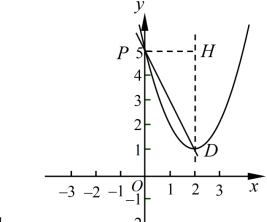
\includegraphics[width=0.82\linewidth]{figures/sol24a.png}}{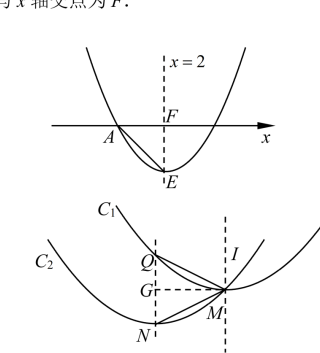
\includegraphics[width=0.9\linewidth]{figures/sol24bc.png}}
\end{teachersolution}

\q{25}\textbf{（本题 14 分，第（1）小题 4 分，第（2）（3）小题各 5 分）}
在 $\triangle ABC$ 中，$\angle BAC\ge90^\circ$，点 $D$ 为边 $AC$ 上一点，$\angle ABD=\angle ACB$，$CD=2$。将 $\triangle ABD$ 沿 $BD$ 翻折得到 $\triangle A_1BD$，点 $A_1$ 恰好落在边 $BC$ 的垂直平分线上。
\subq{1}如图 16，如果点 $A_1$ 在边 $BC$ 上，求 $\dfrac{AD}{AB}$ 的值；
\subq{2}如图 17，如果 $AD=CD$，求 $BD$ 的长；
\subq{3}如果 $AB=CD$，求 $\angle BAC$ 的度数。
\twocolfig{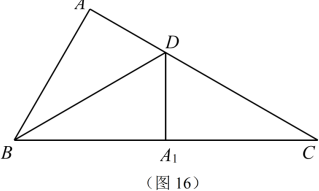
\includegraphics[width=0.78\linewidth]{figures/fig16.png}}{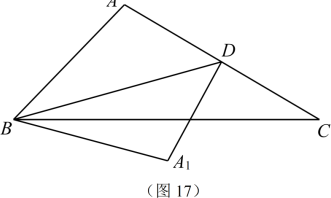
\includegraphics[width=0.82\linewidth]{figures/fig17.png}}
\studentanswer{\answerarea[135mm]}
\begin{teachersolution}
（1）由翻折知 $\triangle ABD\cong\triangle A_1BD$。因 $A_1$ 在 $BC$ 的垂直平分线上，且在 $BC$ 上，所以 $A_1$ 是 $BC$ 的中点。由面积关系可得 $\dfrac{S_{\triangle ABD}}{S_{\triangle ACB}}=\dfrac13$。又 $\angle ABD=\angle ACB$，$\angle BAD$ 为公共角，所以 $\triangle ABD\sim\triangle ACB$。于是
\[
\left(\frac{AD}{AB}\right)^2=\frac13,
\qquad \frac{AD}{AB}=\frac{\sqrt3}{3}.
\]

（2）连接 $AA_1,A_1C$。由 $AD=CD=2$ 得 $A_1B=AB=2\sqrt2$，且 $A_1$ 在 $BC$ 的垂直平分线上，所以 $A_1C=A_1B=2\sqrt2$。设 $BD$ 的垂直平分线与 $AA_1$ 交于 $M$，可得 $DM=\sqrt2$，$AM=\sqrt2$，$BM=\sqrt6$，因此 $BD=BM+DM=\sqrt6+\sqrt2$。

（3）过点 $D$ 作 $DN\parallel AA_1$，交 $A_1C$ 于点 $N$。由相似与黄金分割关系可得
\[
\frac{AD}{CD}=\frac{\sqrt5-1}{2},
\]
进而 $\triangle A_1ND\sim\triangle A_1DC$，得到 $\angle A_1DN=\angle NDC=36^\circ$。又可推出 $\triangle ABA_1$ 为等边三角形，所以 $\angle BAA_1=60^\circ$，且 $\angle CAA_1=36^\circ$。故
\[
\angle BAC=60^\circ+36^\circ=96^\circ.
\]
\fig[0.42\linewidth]{sol25c.png}
\end{teachersolution}

\end{document}
